\documentclass[12pt]{article} 
\usepackage[utf8]{inputenc} 
\usepackage{amsmath}
\usepackage{graphicx}
\usepackage{tikz}
\title{Computer Modeling}
\author{Shimon Panfil}
%\date{} 
 
\begin{document}
\maketitle
\section{What is all about?}
{\em Computer simulation} is a simulation, run on a single computer, or a network of computers, to reproduce behavior of a system. The simulation uses an abstract model (a computer model, or a computational model) to simulate the system. Computer simulations have become a useful part of mathematical modeling of many natural systems in physics (computational physics), astrophysics, climatology, chemistry and biology, human systems in economics, psychology, social science, and engineering. Simulation of a system is represented as the running of the system's model. It can be used to explore and gain new insights into new technology and to estimate the performance of systems too complex for analytical solutions. (Wikipedia)

{\em  Computer modeling} definition: Constructing and manipulating abstract (mathematical and/or graphical) representations of economic, engineering, manufacturing, social, and other types of situations and natural phenomenon, simulated with the help of a computer system. Also called computer simulation.
(http://www.businessdictionary.com/definition/computer-modeling.html)

There are much more definitions and descriptions all of them are pretty useless and circular. However everybody working in high tech industry understand (I hope) what is all about.  Basically computer modeling comprises the following hierarchy of the models:
\begin{description}
\item [Physical model] derived form First Principles (Physical Laws) with the aid of some reasonable assumptions;
\item [Mathematical model] describing the physical one;
\item [Numerical model] comprising algorithms and software for (numerically) solving mathematical model;
\item [Presentation model] comprising UI, methods for information storage and retrieval etc\ldots
\end{description}
The boundaries between models in this scheme are rather artificial and not very clear, the strongest interconnections exits between first two models,
last two are also interleaved. Different parts in this hierarchy are developed in different times and by different (groups of) people with all usual problems of communications, project management and all that. There is also the class of problems specific for computer modeling (and to scientific programming in general) --- we can not easily decide are the results right or wrong and even if know them to be wrong we do not know have the error appeared from programming bug or from bad algorithm or   from mathematical  model inaccuracy or physical model incompleteness (or some combination of above). 



\section{Maxwell's equations}
Light propagation and scattering is a part of classical electrodynamics and as such it is fully described by Maxwell equations. Let us go all way from Maxwell equation in vacuum to our model of light propagation and scattering and fix all the assumptions we need.
In vacuum microscopic Maxwell's equations have the form:
\begin{eqnarray}
	\nabla \times \vec E +\frac{1}{c} \frac{\partial \vec B}{\partial t} &=& 0 \nonumber\\
	\nabla \cdot \vec B &=&0 \nonumber\\
	\nabla \times \vec B -\frac{1}{c} \frac{\partial \vec E}{\partial t} &=& \frac{4\pi}{c} \vec j \nonumber \\
	\nabla \cdot \vec E &=&4\pi \rho \label {micro_me}
\end{eqnarray}
here $\vec E$, $\vec B$ are electric and magnetic fields and $\vec j$ , $\rho$ current and charge densities. I use physical system of units where all fields have the same dimensions, in engineering system SI these equations and all other formulas look slightly differently.

These equations are nice and exact but refer to any particle in our system not even molecules or atoms but every electron and proton. To be practical we should use some averaged fields described collective effects. Averaging does not change homogeneous (first and second) equations in the Maxwell's equation set (\ref{micro_me}) but $\vec B$ is replace by $\vec H$ and $\vec E$ by $\vec D$ in second pair. $\rho$ and $\vec j$ now describe the charges and currents which are external  to the media.
\begin{eqnarray}
	\nabla \times \vec E +\frac{1}{c} \frac{\partial \vec B}{\partial t} &=& 0 \nonumber\\
	\nabla \cdot \vec B &=&0 \nonumber\\
	\nabla \times \vec H -\frac{1}{c} \frac{\partial \vec D}{\partial t} &=& \frac{4\pi}{c} \vec j \nonumber \\
	\nabla \cdot \vec D &=&4\pi \rho \label {me}
\end{eqnarray}
Though equations (\ref{micro_me}) and (\ref{me}) seem very similar they describe completely different physics. Surely we need also so called constituent  equations connecting physical $(\vec E,\vec B)$ and auxiliary fields $(\vec D,\vec H)$. The simplest such equation is 
\begin{eqnarray}
	\vec D&=& \epsilon \vec E \nonumber \\
	\vec j&=& \sigma \vec E \nonumber \\
	\vec B&=& \mu \vec H \label{simple_ce}
\end{eqnarray}
where $\epsilon$,$\sigma$ and $\mu$ are some constants. We shall consider only electrically neutral  ($\rho=0$) and non-magnetic ($\mu=1$) media.

Let us recall that the size of the atom is $\sim 0.1 nm$ and characteristic distance between atoms in molecules is $\sim 0.1-0.2 nm$ so that large polymer molecules have the size comparable with 1 nm. This in turn means that validity of simple constituent equations (\ref{simple_ce}) in  nanometer  scale is not evident and should be checked. Probably the first and second equations  in  (\ref{simple_ce}) should be replaced by anisotropic ones
\begin{eqnarray}
 D_i&=&\epsilon_{jk} E_k \nonumber\\
j_i&=&\sigma_{jk} E_k \label{tensor_ce}
\end{eqnarray}
where tensors $\epsilon_{jk}$ and $\sigma_{jk}$ might be function of coordinates and time.

We may be not interested in transient effects and consider harmonic time dependence only so any time dependent variable can be written as
\begin{equation}
	V(\vec r,t)=v(\vec r) e^{-i\omega t}
\end{equation} 
and Maxwell's equations take the form:
\begin{eqnarray}
	\nabla \times \vec E -\frac{i \omega}{c}  \vec H &=& 0 \nonumber\\
	\nabla \times \vec H +\frac{i \omega n^2(\vec r,\omega)}{c} \vec E &=& 0 \label{harm_me}
\end{eqnarray}
here $n(\vec r,\omega)$ is complex refraction index which determines optical properties of the media. Note that two remaining equations in (\ref {me}) are satisfied automatically on solutions of equations (\ref{harm_me}). 
\begin{eqnarray}
	n(\vec r,\omega)&=&\alpha(\vec r,\omega)+i\beta(\vec r,\omega) \nonumber \\
	\alpha(\vec r,\omega) &>&0 \nonumber \\
	\beta(\vec r,\omega) &\ge & 0 \nonumber \\
	\alpha^2(\vec r,\omega)&=&\frac{\epsilon(\vec r,\omega)}{2}(1+\sqrt{1+\frac{16 \pi^2\sigma^2(\vec r,\omega)}{\omega^2\epsilon^2(\vec r,\omega)}}) \nonumber \\
	\beta^2(\vec r,\omega)&=&\frac{\epsilon(\vec r,\omega)}{2}(-1+\sqrt{1+\frac{16 \pi^2\sigma^2(\vec r,\omega)}{\omega^2\epsilon^2(\vec r,\omega)}}) \label{refrind}
\end{eqnarray}

 It is important also to remember that equations (\ref{harm_me}) and (\ref{refrind}) are obtained with constituent equations (\ref{simple_ce}), on using equations (\ref{tensor_ce}) much more complicated expressions appear. Usually optical media are bad conductors  so $\alpha\gg \beta$. 

To complete the derivation of mathematical model we should add necessary boundary conditions to system (\ref{harm_me}). This mathematical problem can be represented in other of forms e.g. vector wave equation:
\begin{equation}
	\nabla \times \nabla \times  \vec E-\frac{\omega^2 n^2(\vec r,\omega)}{c^2} \vec E=0 \label{vec_wave_eq1}
\end{equation}
which is equivalent to
\begin{eqnarray}
	\nabla^2  \vec E+\frac{\omega^2 n^2(\vec r,\omega)}{c^2} \vec E&=&0 \nonumber \\
	\nabla \cdot \vec E &=&0 \label{vec_wave_eq2}
\end{eqnarray}
It can be also represented as the system of integral equations.

Generally this problem is hopelessly difficult to solve\footnote{Not only becouse of limited computer power but and mainly becouse we can not obtain necessary data}. Fortunately in most of real world problems media may be divided into a number of homogeneous regions where refraction index is constant. So equations (\ref{harm_me},\ref{vec_wave_eq1} or \ref{vec_wave_eq2}) have known analytical solutions. The only (but serious problem) is to apply correct boundary conditions: tangential component of both fields should be continuous for (\ref{harm_me}) and tangential component of electric field together with its normal derivative should be continuous for (\ref{vec_wave_eq1}, \ref{vec_wave_eq2}). Note that the sharp boundary approximation may not be applicable in nanometer scale\footnote {See discussion of molecular size above}. Integral equations are also simplified greatly, all volume integrals disappear, only integral over boundaries survive. 
\section{Boundary Integrals}
Let us describe boundary integrals for arbitrary shaped region with constant refraction index in so called Franz form.
Let V be a region in three dimensional space and S be its boundary. Let $\vec y$ be a point inside V and $\vec x$ be a point on S. Let $\vec \nu(\vec x)$ be internal normal to S.  Let 
\begin{eqnarray}
	\vec E_t(\vec x)&=&\vec \nu(\vec x) \times \vec E(\vec x) \nonumber \\
	\vec H_t(\vec x)&=&\vec \nu(\vec x) \times \vec H(\vec x) \label{tang}
\end{eqnarray}
be tangential component of fields defined on the surface S. It can be proved that these components generate the field 
\begin{eqnarray}
	\vec E(\vec y)&=&\nabla \times \int_S G(R)\vec  E_t(\vec x) ds +\frac{i c}{\omega n^2} \nabla\times\nabla\times\int_S G(R) \vec  H_t(\vec x) ds \nonumber\\
	\vec H(\vec y)&=&\nabla \times \int_S G(R)\vec  H_t(\vec x) ds -\frac{i c}{\omega } \nabla\times\nabla\times\int_S G(R) \vec  E_t(\vec x) ds \label{franz} 
\end{eqnarray}
where 
\begin{eqnarray}
	G(R) &=&\frac{ e^{i \frac{\omega}{c }n R}} {4\pi R} \nonumber \\
	R&=&|\vec x-\vec y| \label{greenf}
\end{eqnarray}
inside the volume V and zero fields outside it.

To complete definition of our models we should formulate more accurately what we mean when we are talking about material boundary. Physically more accurate description would be: there is some thin intermediate layer where bulk material properties change their values. We can {\bf assume} that the thickness of these intermediate layers are all much smaller than minimal characteristic dimension of our problem (e.g. light wavelength) and results do not depend on what exactly is going inside or near intermediate layers. However this assumption only tells us nothing about the shape and position of the boundary: e.g. is it plane, curved , rough  etc\ldots  {\em Boundary properties are fixed by additional assumptions and their correctness should be checked.}  Putting this in other words it is "effective boundary" and its location and shape need not be exactly same as that of geometric boundary which is not defined at nanometer scale. Note that sharp angles and other non-smooth parts of boundary lead to the field singularities and bad convergence.
%\begin{figure}[h]
%    \centering
%   \begin{tikzpicture}[domain=0:4] 
%    \draw[very thin,color=gray] (-0.1,-1.1) grid (3.9,3.9);
%    \draw[->] (-0.2,0) -- (4.2,0) node[right] {$x$}; 
%    \draw[->] (0,-1.2) -- (0,4.2) node[above] {$f(x)$};
%    \draw[color=red]    plot (\x,\x)             node[right] {$f(x) =x$}; 
%    \draw[color=blue]   plot (\x,{sin(\x r)})    node[right] {$f(x) = \sin x$}; 
%    \draw[color=orange] plot (\x,{0.05*exp(\x)}) node[right] {$f(x) = \frac{1}{20} \mathrm e^x$};
%  \end{tikzpicture}
%    \caption{Transition layer and effective boundary}
%    \label{fig:effb}
%\end{figure}
  
\begin{figure}[h]
    \centering
   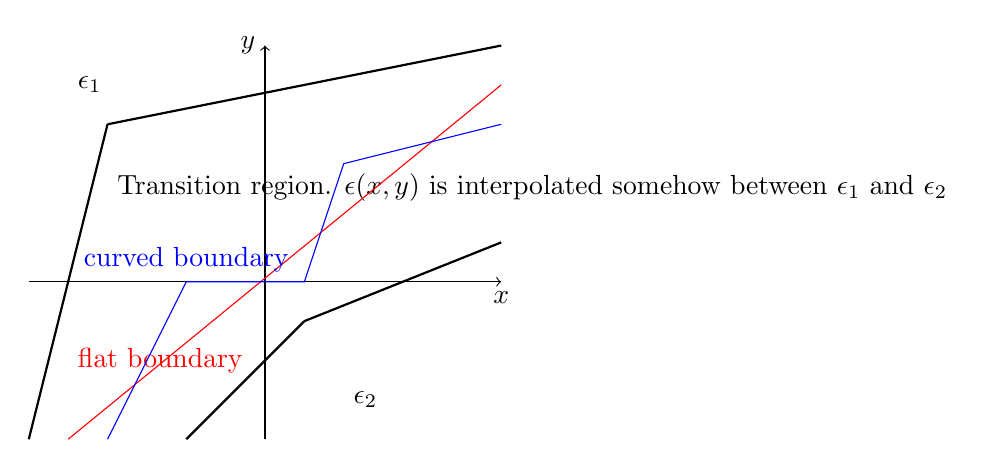
\begin{tikzpicture}[scale=1.0]
% Draw thin grid lines with color 40% gray + 60% white auxiliary
%\draw [step=0.5,thin,gray!40] (-3.0,-2.0) grid (3.0,3.0);

% Draw x and y axis lines
\draw [->] (-3.0,0) -- (3.0,0) node [below] {$x$};
\draw [->] (0,-2.0) -- (0,3.0) node [left] {$y$};
%Draw region1
\draw (-2.5,2.5) node [right] {$\epsilon_1$};
\draw [thick] (-3.0,-2.0) -- (-2.0,2.0);
\draw [thick] (-2.0,2.0) -- (3.0,3.0);
%Draw region2
\draw [thick] (-1.0,-2.0) -- (0.5,-0.5);
\draw [thick] (0.5,-0.5) -- (3.0,0.5);
\draw (1.0,-1.5) node [right] {$\epsilon_2$};
\draw (-2.0,1.2) node[right] {Transition region. $\epsilon(x,y)$  is interpolated somehow between $\epsilon_1$  and $\epsilon_2$};
%Draw flat boundary
\draw[color=red] (-2.5,-2.0) --(3.0,2.5);
\draw[color=red] (-2.5,-1.0) node [right] {flat boundary};
%draw curved boundary
\draw [color=blue]  
   (-2.0,-2.0) to  (-1.0,0.0) 
   to (0.5,0.0) 
   to (1.0,1.5) 
   to (3.0,2.0) ;
\draw[color=blue] (-1.0,0.0) node [above] {curved boundary};
  \end{tikzpicture}
    \caption{Transition layer and effective boundary}
    \label{fig:effb}
\end{figure}
\section{Algorithms and Methods}
Let us suppose that me managed to divide our volume of interest into a number of parts with constant refraction indices and the condition that allow to neglect transition layers are fulfilled. We can use quite a few methods to solve the equations (\ref{harm_me}) or (\ref{franz}). Let us consider them briefly.
\subsection{RCWA}
\begin{quotation}
Rigorous coupled-wave analysis (RCWA) is a semi-analytical method in computational electromagnetics that is most typically applied to solve scattering from periodic dielectric structures. It is a Fourier-space method so devices and fields are represented as a sum of spatial harmonics. The method is based on the Floquet's theorem that the solutions of periodic differential equations can be expanded with Floquet functions (or sometimes referred as Bloch wave, especially in solid-state physics community). A device is divided into layers that are each uniform in the z direction. A staircase approximation is needed for curved devices with properties such as dielectric permittivity graded along the z-direction. The electromagnetic modes in each layer are calculated and analytically propagated through the layers. The overall problem is solved by matching boundary conditions at each of the interfaces between the layers using a technique like scattering matrices. To solve for the electromagnetic modes, which are decided by the wave vector of the incident plane wave, in periodic dielectric medium, the Maxwell's equations (in partial differential form) as well as the boundary conditions are expanded by the Floquet functions and turned into infinitely large algebraic equations. With the cutting off of higher order Floquet functions, depending on the accuracy and convergence speed one needs, the infinitely large algebraic equations become finite and thus solvable by computers.

Being a Fourier-space method it suffers several drawbacks. Gibbs phenomenon is particularly severe for devices with high dielectric contrast. Truncating the number of spatial harmonics can also slow convergence and techniques like fast Fourier factorization (FFF) should be used. FFF is straightforward to implement for 1D gratings, but the community is still working on a straightforward approach for crossed grating devices. The difficulty with FFF in crossed grating devices is that the field must be decomposed into parallel and perpendicular components at all of the interfaces. This is not a straightforward calculation for arbitrarily shaped devices.

Boundary conditions must be enforced at the interfaces between all the layers. When many layers are used, this becomes too large to solve simultaneously. Instead, we borrow from network theory and calculate scattering matrices. This lets us solve the boundary conditions one layer at a time. 
\end{quotation}
This long quotation from Wikipedia  describes the method well enough. I would like only add some comments. All interfaces should be exactly plane and parallel and all structures should be exactly periodical this is both advantage --- no need to tune the method for particular case and disadvantage also --- we can not model even small deviations. Staircase approximation may produce severe artifacts I will not explain all the theory behind but show simple example . Let us make staircase approximation for the hypotenuse of right triangle, see fig. (\ref{fig:rtrg}), if we compute the area of triangle all is fine, but on computing the length of hypotenuse we will get that it is sum of catheti!
\begin{figure}[h]
    \centering
   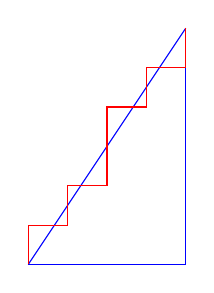
\begin{tikzpicture}[scale=1.0]
% Draw thin grid lines with color 40% gray + 60% white auxiliary
%\draw [step=0.5,thin] (0,0) grid (2.0,3.0);
% Draw triangle
\draw [color=blue] (0,0) -- (2.0,0);
\draw [color=blue] (2.0,0) -- (2.0,3.0);
\draw [color=blue] (0,0) -- (2.0,3.0);
\draw [color=red] (0.0,0.0) -- (0.0,0.5) -- (0.5,0.5) -- (0.5,1.0) -- (1.0,1.0) --(1.0,2.0) --(1.5,2.0) --(1.5,2.5) --(2.0,2.5) --(2.0,3.0);

  \end{tikzpicture}
    \caption{Right triangle}
    \label{fig:rtrg}
\end{figure}
\subsection{FDFD}
Finite Differences Frequency Domain (FDFD) method is based on finite difference approximation of differential equations (\ref{harm_me}) or (\ref{vec_wave_eq1}) \footnote{Actually any differential equation}. So the equation at hands takes the form $A x=b$, where matrix $A$ is large but sparse. Feasibility and efficiency of the method really are that of software for working with sparse matrices. Good open source (e.g. SuperLU http://crd-legacy.lbl.gov/~xiaoye/SuperLU/ )and commercial packages do exist. 
\subsection{DDA}
The discrete dipole approximation (DDA) is a method for computing scattering of radiation by particles of arbitrary shape and by periodic structures. Simply stated, the DDA is an approximation of the continuum target by a finite array of polarizable points. The points acquire dipole moments in response to the local electric field. For a finite array of point dipoles the scattering problem may be solved exactly, so the only approximation that is present in the DDA is the replacement of the continuum target by an array of N-point dipoles. The replacement requires specification of both the geometry (location of the dipoles) and the dipole polarizabilities. For monochromatic incident waves the self-consistent solution for the oscillating dipole moments may be found; from these the absorption and scattering cross sections are computed. If DDA solutions are obtained for two independent polarizations of the incident wave, then the complete amplitude scattering matrix can be determined. DDA may be considered as particular sort of Finite Volume Element Method. Good open source exists (http://www.ddscat.org/)
\subsection{BEM}
Boundary Element Method (BEM) is simply  discretization of surface integral equations (\ref{franz}) or similar ones. Matrices which appear in BEM are considerably smaller than that in FDFD or FEM but they are not sparse. Well known software packages e.g. LAPACK exist for such matrices.
\section{Physical Optics}
In previous sections we consider optics as particular case of electromagnetic problem, nothing special was used. It is well known however that for most practical problems the solution of Maxwell's equation is not feasible and some kind of physically motivated approximation is needed. The simplest and most used approximation is geometrical optics where wave properties of light are neglected completely. Physical optics is next in line, it takes wave properties in consideration only when it is necessary: e.g. when the distance from the boundary is of order of wave length (diffraction) or we trying to see something which has size comparable with wave length. Mathematically speaking physical optics is short wave length approximation to Maxwell's equations. The most natural form of such approximation is so called eikonal equations.

\end{document}
